%\VignetteIndexEntry{CSFA: Vignette Example Analysis} \\
%\VignetteDepends{CSFA}
%\VignettePackage{CSFA}
%\VignetteEngine{knitr::knitr}
\documentclass[a4paper]{article}\usepackage[]{graphicx}\usepackage[]{color}
%% maxwidth is the original width if it is less than linewidth
%% otherwise use linewidth (to make sure the graphics do not exceed the margin)
\makeatletter
\def\maxwidth{ %
  \ifdim\Gin@nat@width>\linewidth
    \linewidth
  \else
    \Gin@nat@width
  \fi
}
\makeatother

\definecolor{fgcolor}{rgb}{0.345, 0.345, 0.345}
\newcommand{\hlnum}[1]{\textcolor[rgb]{0.686,0.059,0.569}{#1}}%
\newcommand{\hlstr}[1]{\textcolor[rgb]{0.192,0.494,0.8}{#1}}%
\newcommand{\hlcom}[1]{\textcolor[rgb]{0.678,0.584,0.686}{\textit{#1}}}%
\newcommand{\hlopt}[1]{\textcolor[rgb]{0,0,0}{#1}}%
\newcommand{\hlstd}[1]{\textcolor[rgb]{0.345,0.345,0.345}{#1}}%
\newcommand{\hlkwa}[1]{\textcolor[rgb]{0.161,0.373,0.58}{\textbf{#1}}}%
\newcommand{\hlkwb}[1]{\textcolor[rgb]{0.69,0.353,0.396}{#1}}%
\newcommand{\hlkwc}[1]{\textcolor[rgb]{0.333,0.667,0.333}{#1}}%
\newcommand{\hlkwd}[1]{\textcolor[rgb]{0.737,0.353,0.396}{\textbf{#1}}}%

\usepackage{framed}
\makeatletter
\newenvironment{kframe}{%
 \def\at@end@of@kframe{}%
 \ifinner\ifhmode%
  \def\at@end@of@kframe{\end{minipage}}%
  \begin{minipage}{\columnwidth}%
 \fi\fi%
 \def\FrameCommand##1{\hskip\@totalleftmargin \hskip-\fboxsep
 \colorbox{shadecolor}{##1}\hskip-\fboxsep
     % There is no \\@totalrightmargin, so:
     \hskip-\linewidth \hskip-\@totalleftmargin \hskip\columnwidth}%
 \MakeFramed {\advance\hsize-\width
   \@totalleftmargin\z@ \linewidth\hsize
   \@setminipage}}%
 {\par\unskip\endMakeFramed%
 \at@end@of@kframe}
\makeatother

\definecolor{shadecolor}{rgb}{.97, .97, .97}
\definecolor{messagecolor}{rgb}{0, 0, 0}
\definecolor{warningcolor}{rgb}{1, 0, 1}
\definecolor{errorcolor}{rgb}{1, 0, 0}
\newenvironment{knitrout}{}{} % an empty environment to be redefined in TeX

\usepackage{alltt}
\usepackage{etex}
%\usepackage{Sweave}
\usepackage[margin=2cm]{geometry}
\usepackage{graphicx}
\usepackage{amsmath}
\usepackage{amssymb}
\usepackage{color}
\usepackage{easybmat}
\usepackage{setspace}
\usepackage{subcaption}
\usepackage{multirow}
\usepackage{float}
\usepackage[english]{babel}
\usepackage{natbib}

\usepackage{hyperref}
\hypersetup{
	colorlinks, 
	citecolor=black,
	filecolor=black,
	linkcolor=black,
	urlcolor=black
}

\usepackage{subcaption}

\title{CSFA 0.1 - Vignette}
\date{}
\author{Ewoud De Troyer}
\IfFileExists{upquote.sty}{\usepackage{upquote}}{}
\begin{document}
\maketitle
\section{Introduction}

One of the many challenges in today's omics data is the goal of connecting those
compounds/molecules/samples together which have similar properties by gene
expression.
Techniques like this allow the discovery of new molecule properties by
connecting their signatures with those derived from already well-known ones.\\
Papers such as \citet{Lamb2006} and \citet{Zhang2008} both already took up the
challenge of dealing with this problem. In \citet{Lamb2006}, a reference
collection of gene expression profiles from human cells treated with bioactive
small molecules was created in order to design a systematic approach to discover
these functional connections. While their approach achieved a good degree of
succes, it was unable to measure statistical significance. This is where the
paper from \citet{Zhang2008} continued for example. Their paper offers a more
principled statistical procedure to test connections between the compounds which allows the valuation of statistical significance.
\\ \\
The CSFA package accompanies the paper/report by Shkedy, Z. and De Troyer. E. (ADD REAL REF),
which proposes the usage of {\it factor analysis} methods (Principal Component
Analysis (=PCA), (Sparse) Multiple Factor Analysis (MFA) \citep{Abdi2013} and
FABIA (Factor Analysis for Bicluster Acquisition) \citep{Hochreiter2010}) to
derive the connectivity between compounds.
Using these methods, not only do you obtain information about the connectivity between the compounds, you also get
information about which genes are responsible for guiding this connectivity.\\
Further instead of computing a pairwise correlation/connection score between the
compounds, now the entire available data is being used to look for dominant structures on both dimenstions. This is very similar to try to discover biclusters in the data. Consequently, it is not necessary anymore to decide upon a cut-off for up- and downregulated genes since you will be using all the genes to do the factor analysis.
\\
It should also be noted that the setting in which the {\it factor analysis} is
applied, is slightly different from the one in the Connectivity Map
\citep{Lamb2006}.
In the Connectivity Map there is a large data set of references profiles to
which the query signatures are compared. In this setting, the meaning of
`reference` and `query` will be switched around. You start with a small set of
references, namely a small set of samples of which they are similar. These are compared with a larger set of queries in order to try to discover samples or compounds similar to the reference set. \\
Further, since the methods will be applied on a matrix which consists out of
both the reference and the query profiles, the number of genes for these signatures will have to be the same.
\begin{equation}\label{eq:structure}
\begin{BMAT}{c}{cc}
	\begin{BMAT}{ccc}{c}
		\overbrace{\left[\begin{BMAT}(@,50pt,80pt){c:}{c}
		\mathbf{X}_1\\
		\end{BMAT}\right.}^{Reference\ Samples}
		&
		\overbrace{\left.\begin{BMAT}(@,80pt,80pt){c}{c}
		\mathbf{X}_2\\
		\end{BMAT}\right]}^{Query\ Samples}
		&
		\begin{BMAT}{c}{c}
		g \text{ genes}
		\end{BMAT}
	\end{BMAT}
	\\
	\begin{BMAT}{l}{c}
		n \text{ samples}\\
	\end{BMAT}
\end{BMAT}
\end{equation}
Finally in order to easily compare these methods with the Zhang and Gant Score,
CSFA also includes an implementation of this algorithm together with the ability
to compare the scores with the FA scores.
\section{Data}
In order to showcase the functionality of CSFA, some simulated microarray data
will be used. The data contains 1000 genes and 341 compounds of which 6 will be used as
reference signatures. The remaining query signatures consist out of 5 strongly
positive connected compounds, 20 weakly positive connected compounds, 10
strongly negative connected compounds and 300 compounds which are not connected
at all.



\begin{knitrout}
\definecolor{shadecolor}{rgb}{0.969, 0.969, 0.969}\color{fgcolor}\begin{figure}[H]

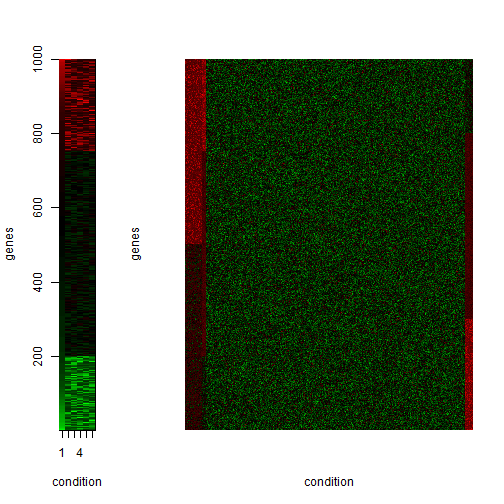
\includegraphics[width=\maxwidth]{figure/data_heatmap-1} \caption[Heatmap of Reference and Query Matrix]{Heatmap of Reference and Query Matrix\label{fig:data_heatmap}}
\end{figure}


\end{knitrout}
%also add image plot of data


\section{Example CS Analysis}
Start by first loading both the CSFA library and the example data available
in the package. The simulated data is split up in the reference and query
matrix.

\begin{knitrout}
\definecolor{shadecolor}{rgb}{0.969, 0.969, 0.969}\color{fgcolor}\begin{kframe}
\begin{alltt}
        \hlkwd{library}\hlstd{(CSFA)}
        \hlkwd{data}\hlstd{(}\hlstr{"dataSIM"}\hlstd{,}\hlkwc{package}\hlstd{=}\hlstr{"CSFA"}\hlstd{)}

        \hlstd{refMat} \hlkwb{<-} \hlstd{dataSIM[,}\hlkwd{c}\hlstd{(}\hlnum{1}\hlopt{:}\hlnum{6}\hlstd{)]}
        \hlstd{querMat} \hlkwb{<-} \hlstd{dataSIM[,}\hlopt{-}\hlkwd{c}\hlstd{(}\hlnum{1}\hlopt{:}\hlnum{6}\hlstd{)]}
\end{alltt}
\end{kframe}
\end{knitrout}

\noindent Next, the Connectivity Scores from Zhang and Gant, MFA and FABIA will
be computed with the package. The last two methods will also provide scores for the
genes involved in the structure.\\
More details about the connectivity and gene scores as well as the decision
making of which component to look at can be be found in Shkedy, Z. and De
Troyer, E. (ADD REF).

\subsection{Zhang and Gant}
The Zhang and Gant scores are computed with the default parameters. This means
all the genes will be used (no cut-off) and the query signature will be
considered as an ordered signature. Also no permutation will be applied by
default.
\\Note that for the vignette, which is a
sweave document, we use the "sweave" \texttt{plot.type}. Normally you would be
using either "device" or "pdf".

\begin{knitrout}
\definecolor{shadecolor}{rgb}{0.969, 0.969, 0.969}\color{fgcolor}\begin{kframe}
\begin{alltt}
        \hlstd{out_ZG} \hlkwb{<-} \hlkwd{CSanalysis}\hlstd{(refMat,querMat,}\hlstr{"CSzhang"}\hlstd{,}\hlkwc{plot.type}\hlstd{=}\hlstr{"sweave"}\hlstd{)}
\end{alltt}
\begin{verbatim}
##    posname  posscore negname    negscore
## 1    cSP-7 0.8159043   cSN-6 -0.74898237
## 2   cSP-10 0.8137249   cSN-8 -0.74288930
## 3    cSP-9 0.8093167   cSN-3 -0.73490411
## 4    cSP-8 0.8081590   cSN-2 -0.73414170
## 5    cSP-6 0.8081177  cSN-10 -0.73401815
## 6   cWP-17 0.5702188   cSN-7 -0.72983443
## 7   cWP-19 0.5694001   cSN-1 -0.72942985
## 8   cWP-12 0.5672755   cSN-9 -0.72934793
## 9   cWP-11 0.5659705   cSN-4 -0.72832312
## 10   cWP-7 0.5658364   cSN-5 -0.72709705
## 11   cWP-4 0.5649765    c-25 -0.03391145
## 12   cWP-9 0.5648644   c-264 -0.03185064
## 13   cWP-3 0.5621351    c-28 -0.03167404
## 14   cWP-1 0.5590061    c-16 -0.03005021
## 15   cWP-8 0.5581202   c-220 -0.02962786
## 16   cWP-5 0.5578107    c-32 -0.02801159
## 17  cWP-18 0.5485421    c-94 -0.02700210
## 18  cWP-15 0.5481818    c-27 -0.02650816
## 19  cWP-16 0.5473567   c-228 -0.02583543
## 20   cWP-2 0.5473340   c-169 -0.02576697
\end{verbatim}
\end{kframe}\begin{figure}[H]


{\centering 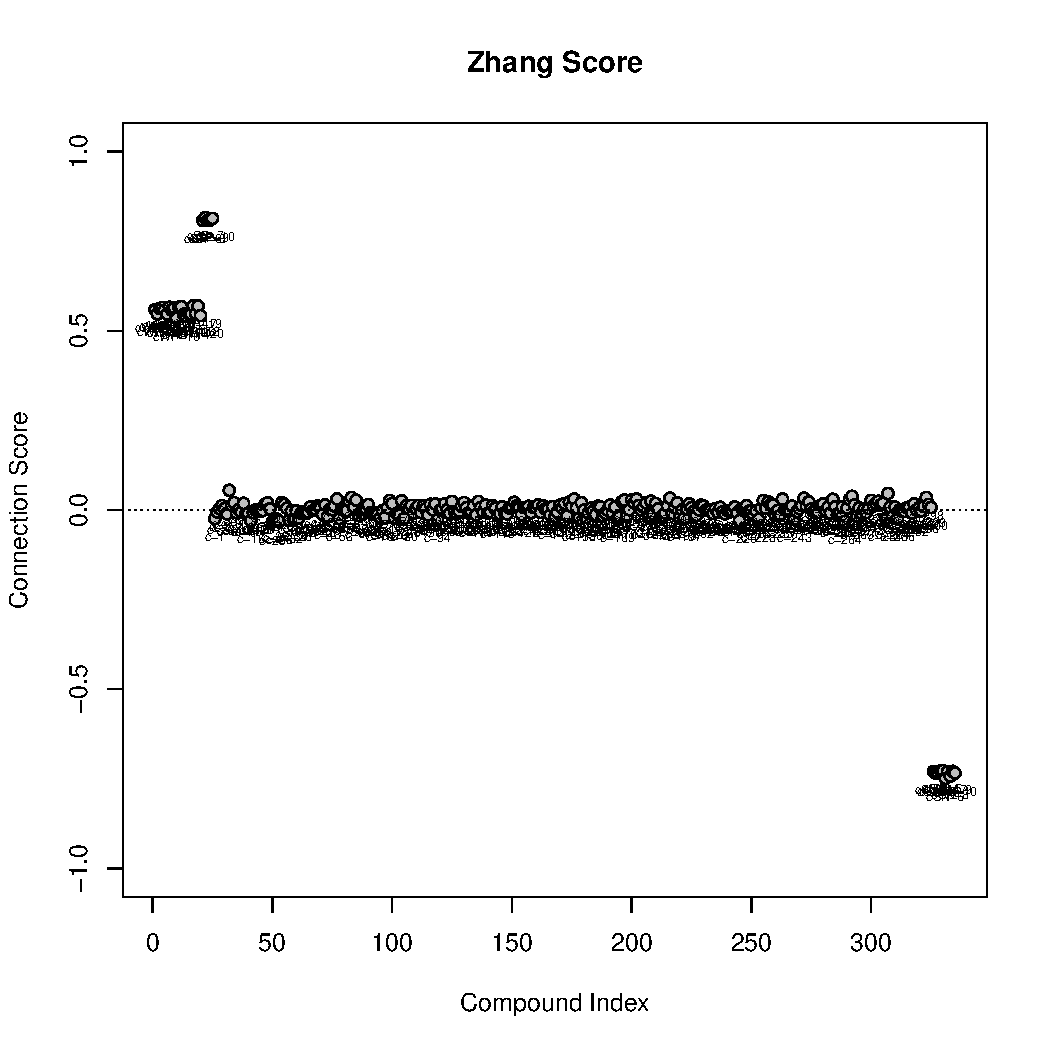
\includegraphics[width=11cm]{figure/ZG-1} 

}

\caption[CSanalysis Graphs for CSzhang]{CSanalysis Graphs for CSzhang\label{fig:ZG}}
\end{figure}


\end{knitrout}

\noindent While all the connectivity scores can be found in the \texttt{out\_ZG}
object, the function already prints by default the top 20 positive and negative
connectivity scores. Figure \ref{fig:ZG} clearly shows the positive (weak and
strong) and negative connected compounds.

\subsection{MFA}
The next CS analysis which is applied is the one using Multiple Factor Analysis
(MFA) by setting the \texttt{type} to \texttt{"CSmfa"}. Three of the
available plots were chosen, namely the Reference Loadings, Gene Scores,
Compound Loadings (Connectivity Scores) and Compound Profiles
(\texttt{which=c(2,4,5)}).\\
Note that in the R-code we already preselected which component to investigate
with \texttt{factor.plot}.
Further we also already decided which columns of the query matrix we would like
to draw in the compound profiles graph with \texttt{column.interest}. Indices 1, 2 and 3 coincide
with 3 weakly positive connected compounds.\\ \\
However, if you are not sure beforehand what you want to investigate, you can
also decide upon these parameters on the fly interactively. To do this simply
set these parameters to \texttt{NULL} or leave them out.\\
To determine \texttt{factor.plot}, you will be able to to click on the factor
you want to observe in the {\it "Loadings for Ref..."} plot. After all, this graph will be
your main guideline on which factor is capturing the structure of your reference
set of signatures. As shown in Figure \ref{fig:MFA} below, this is clearly the
first factor. \\
Next, the \texttt{column.interest} parameter can be chosen in the {\it "Compound
Loadings"} plot. You can left-click on multiple compounds you wish to draw in
the compound profiles graph (and right-click to stop the selection procedure). 

\begin{knitrout}
\definecolor{shadecolor}{rgb}{0.969, 0.969, 0.969}\color{fgcolor}\begin{kframe}
\begin{alltt}
        \hlstd{out_MFA} \hlkwb{<-} \hlkwd{CSanalysis}\hlstd{(refMat,querMat,}\hlstr{"CSmfa"}\hlstd{,}\hlkwc{plot.type}\hlstd{=}\hlstr{"sweave"}\hlstd{,}\hlkwc{which}\hlstd{=}\hlkwd{c}\hlstd{(}\hlnum{2}\hlstd{,}\hlnum{4}\hlstd{,}\hlnum{5}\hlstd{),}
                        \hlkwc{factor.plot}\hlstd{=}\hlnum{1}\hlstd{,}\hlkwc{column.interest}\hlstd{=}\hlkwd{c}\hlstd{(}\hlnum{1}\hlstd{,}\hlnum{2}\hlstd{,}\hlnum{3}\hlstd{))}
\end{alltt}
\begin{verbatim}
## Echoufier Rv Correlation:
##           Reference     Query       MFA
## Reference 1.0000000 0.4947578 0.8001384
## Query     0.4947578 1.0000000 0.9171329
## MFA       0.8001384 0.9171329 1.0000000
\end{verbatim}
\end{kframe}\begin{figure}[H]


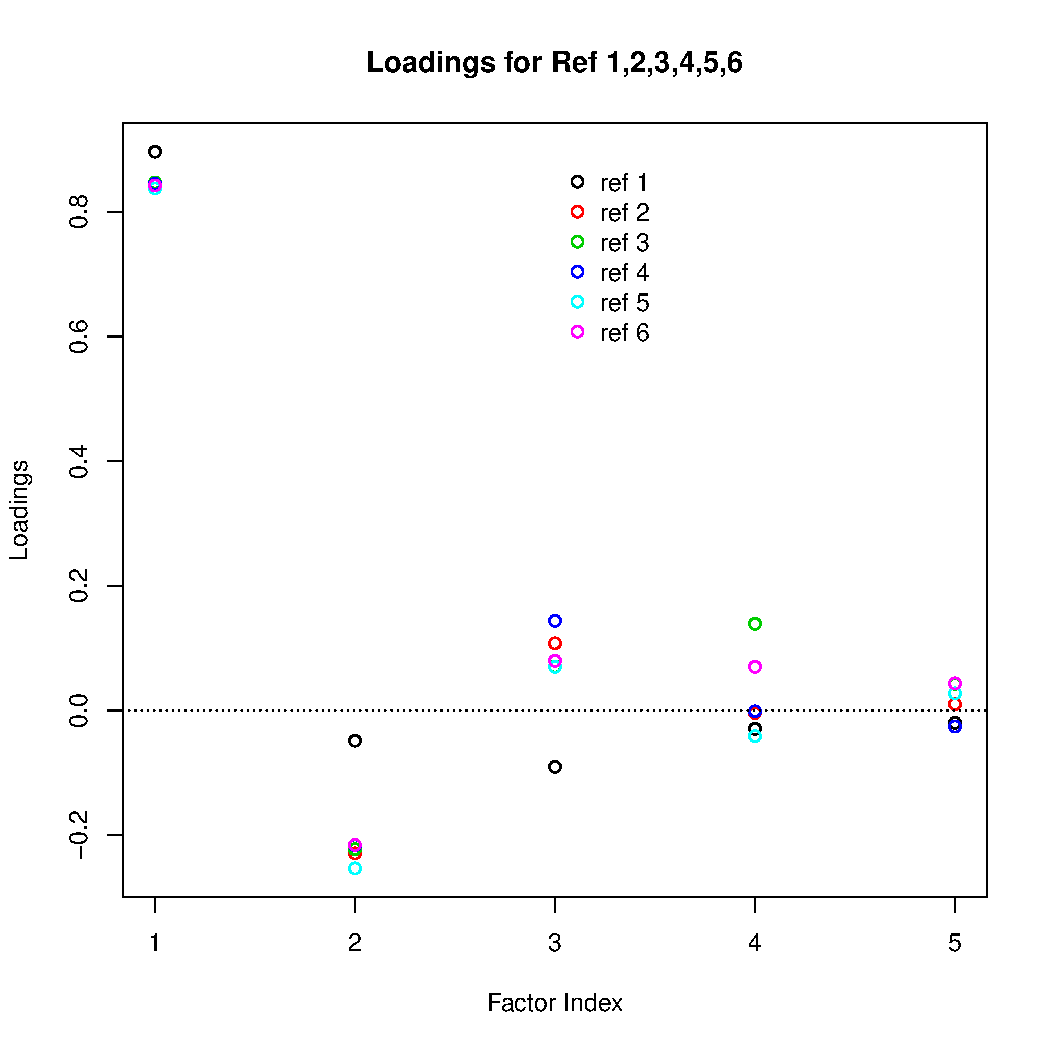
\includegraphics[width=9cm,height=10cm]{figure/MFA-1} 
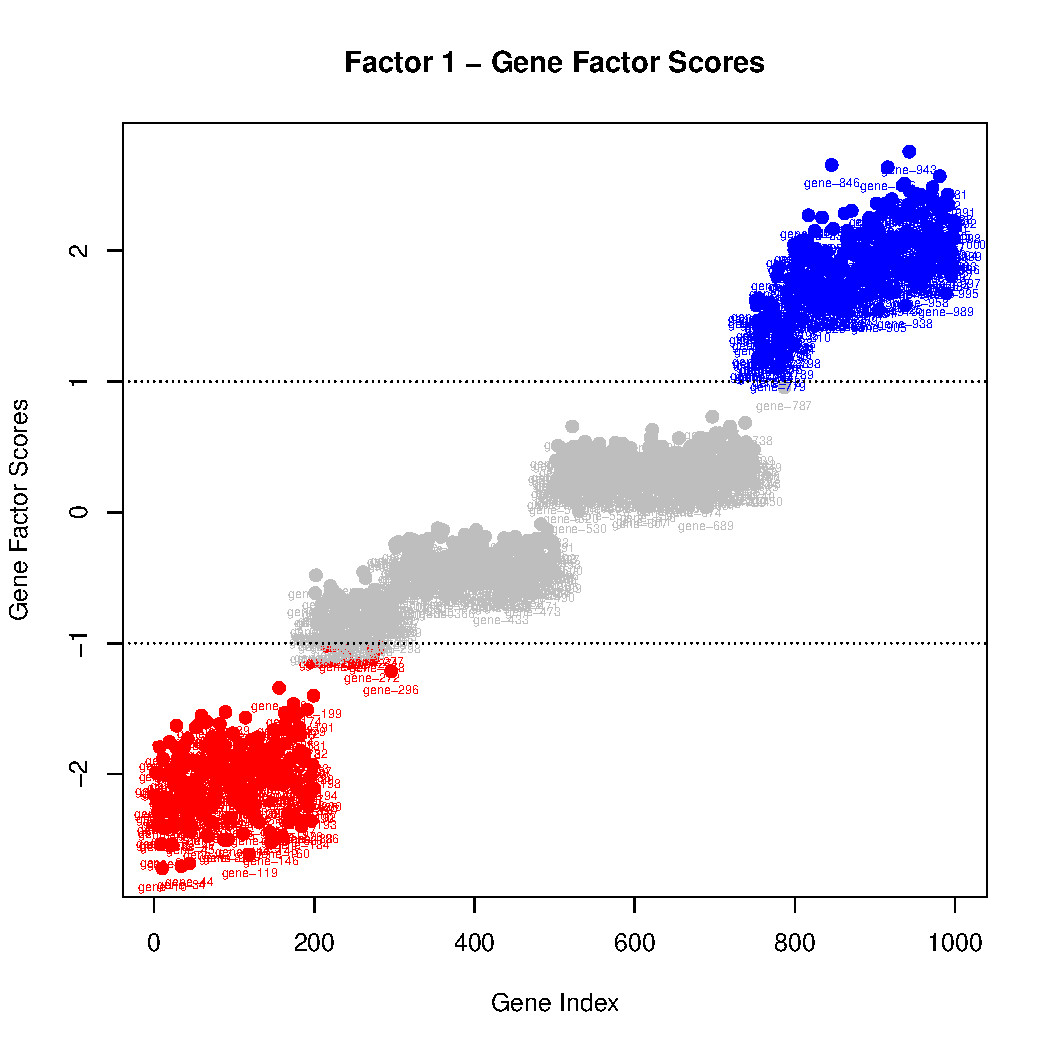
\includegraphics[width=9cm,height=10cm]{figure/MFA-2} 
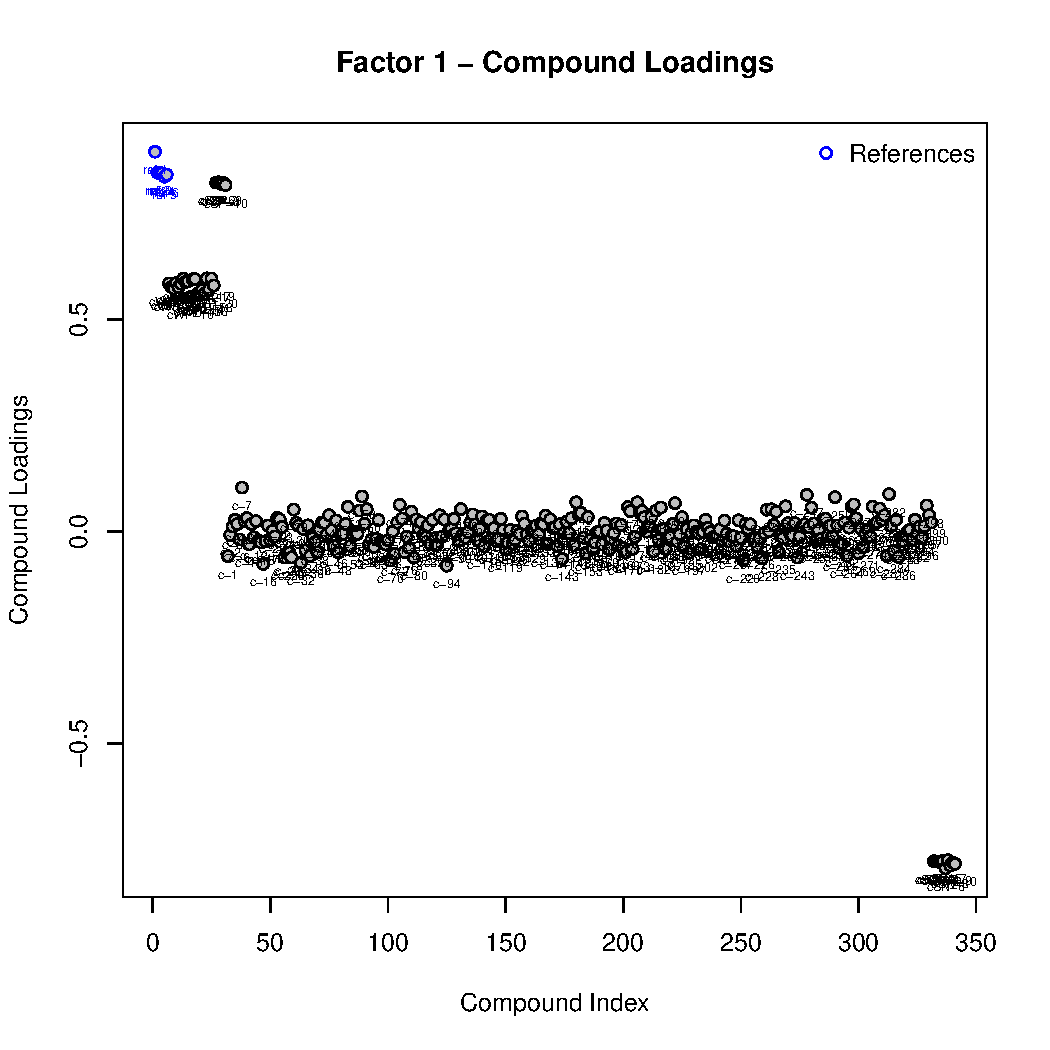
\includegraphics[width=9cm,height=10cm]{figure/MFA-3} 
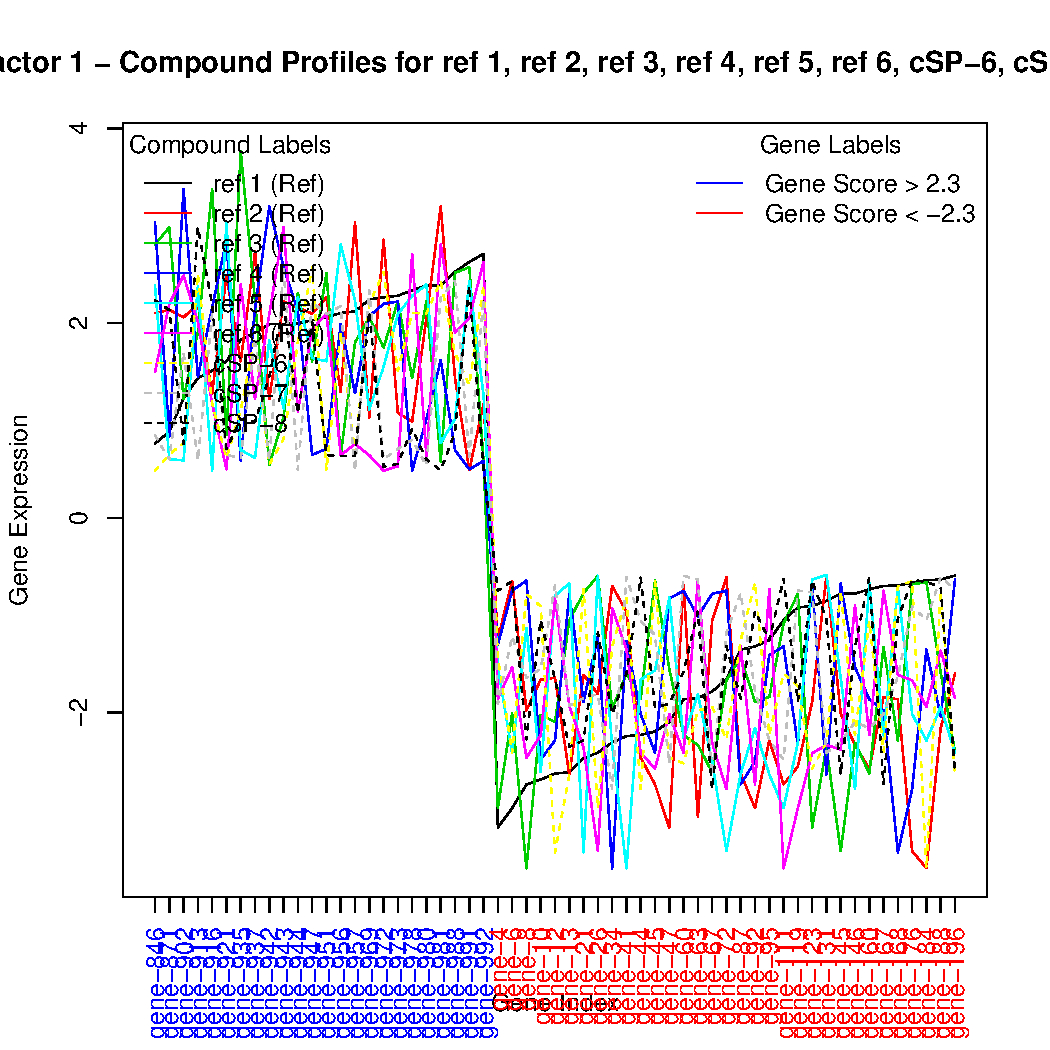
\includegraphics[width=9cm,height=10cm]{figure/MFA-4} \hfill{}

\caption[CSanalysis Graphs for CSfma]{CSanalysis Graphs for CSfma\label{fig:MFA}}
\end{figure}


\end{knitrout}

\noindent Just like in the Zhang and Gant plot, we again see that the simulated
positive and negative connected compounds are appearing in the Compound Loadings
plot. However now we also get a plot showing the scores of the genes involved in
the structure of the first factor in the MFA analysis.\\
Finally also note that the \texttt{CSanalysis} function automatically prints the
Echoufier Rv Correlation matrix between the Reference, Query and MFA matrix.
%fig.keep="high",fig.pos='H',fig.show='hold',out.width='9cm',out.height='10cm',fig.align='left'
%show plots, but also explain how interactivity works


\subsection{FABIA}
The last analysis is done with FABIA, Factor Analysis for Bicluster Acquisition
(\texttt{type="CSfabia"}). We will only select 2 plots this time, namely the
reference loadings and compound loadings (\texttt{which=c(2,5)}). However in
contrary with the MFA anaylsis, we can select 2 components for this analysis.
Based on the reference loadings we decide to select bicluster 1 and 2
(\texttt{BC.plot=c(1,2)}). \\
This time we also do some manual coloring of the columns to highlight some
strongly connected compounds with \texttt{color.columns}. We start by making a vector of length
341 (column dimension of example data) and fill it with the color black. Next we fill in the
color blue for the 6 reference compounds and red for 3 of the strongly positive
connected compounds. We also change the legend according to this coloring.\\ \\
Note that we have also set a seed just before the FABIA analysis in order to
have a reproducible result.

%can use multiple BC for fabia
\begin{knitrout}
\definecolor{shadecolor}{rgb}{0.969, 0.969, 0.969}\color{fgcolor}\begin{kframe}
\begin{alltt}
        \hlstd{color.columns} \hlkwb{<-} \hlkwd{rep}\hlstd{(}\hlstr{"black"}\hlstd{,}\hlkwd{dim}\hlstd{(dataSIM)[}\hlnum{2}\hlstd{])}
        \hlstd{color.columns[}\hlnum{1}\hlopt{:}\hlnum{6}\hlstd{]} \hlkwb{<-} \hlstr{"blue"}
        \hlstd{color.columns[}\hlkwd{c}\hlstd{(}\hlnum{29}\hlstd{,}\hlnum{30}\hlstd{,}\hlnum{31}\hlstd{)]} \hlkwb{<-} \hlstr{"red"}

        \hlkwd{set.seed}\hlstd{(}\hlnum{8956}\hlstd{)}
        \hlstd{out_FABIA} \hlkwb{<-} \hlkwd{CSanalysis}\hlstd{(refMat,querMat,}\hlstr{"CSfabia"}\hlstd{,}\hlkwc{plot.type}\hlstd{=}\hlstr{"sweave"}\hlstd{,}\hlkwc{which}\hlstd{=}\hlkwd{c}\hlstd{(}\hlnum{2}\hlstd{,}\hlnum{5}\hlstd{),}
                        \hlkwc{color.columns}\hlstd{=color.columns,}
                        \hlkwc{legend.names}\hlstd{=}\hlkwd{c}\hlstd{(}\hlstr{"References"}\hlstd{,}\hlstr{"SP Connected"}\hlstd{),}
                        \hlkwc{legend.cols}\hlstd{=}\hlkwd{c}\hlstd{(}\hlstr{"blue"}\hlstd{,}\hlstr{"red"}\hlstd{),} \hlkwc{BC.plot}\hlstd{=}\hlkwd{c}\hlstd{(}\hlnum{1}\hlstd{,}\hlnum{2}\hlstd{),}
                        \hlkwc{gene.thresP}\hlstd{=}\hlnum{2}\hlstd{,}\hlkwc{gene.thresN}\hlstd{=}\hlopt{-}\hlnum{2}\hlstd{)}
\end{alltt}
\end{kframe}\begin{figure}[H]


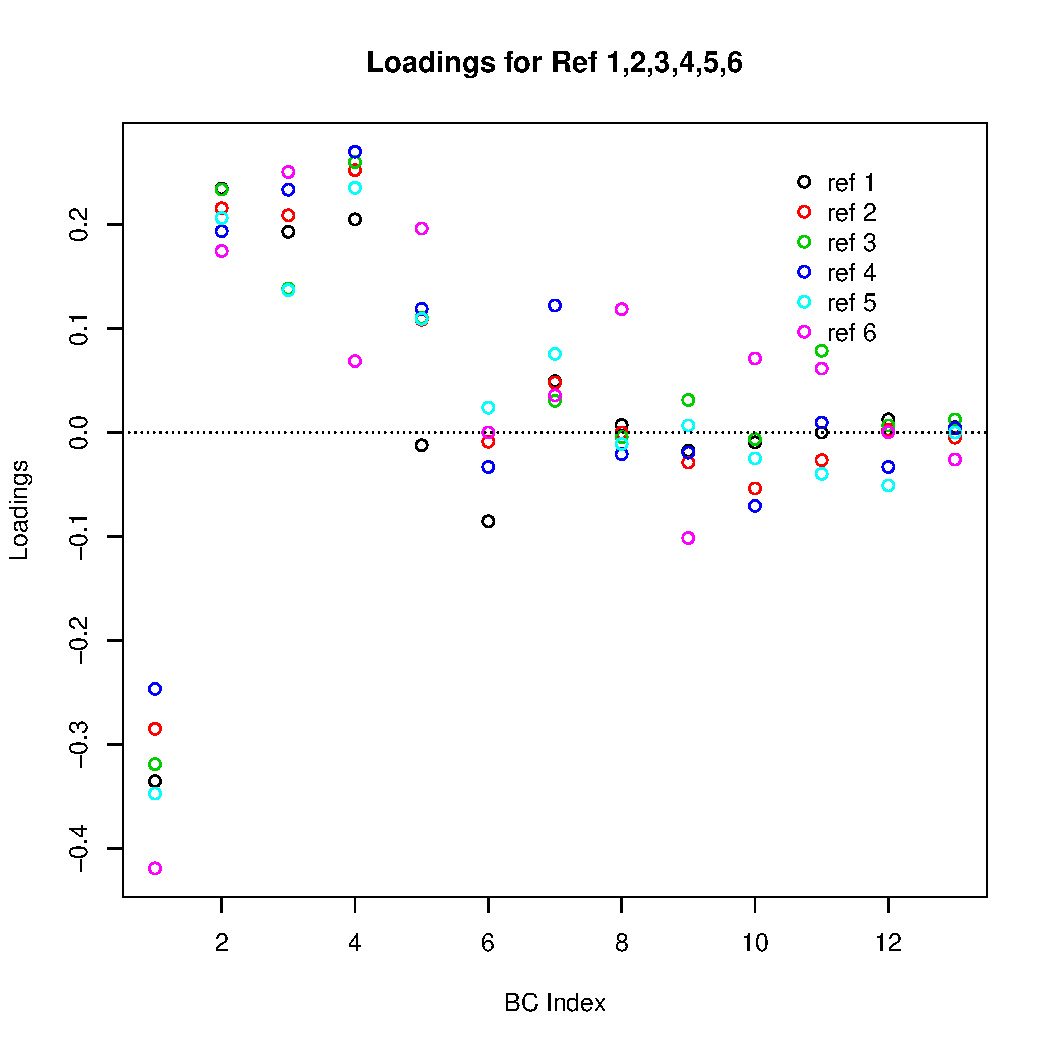
\includegraphics[width=9cm,height=10cm]{figure/FABIA-1} 
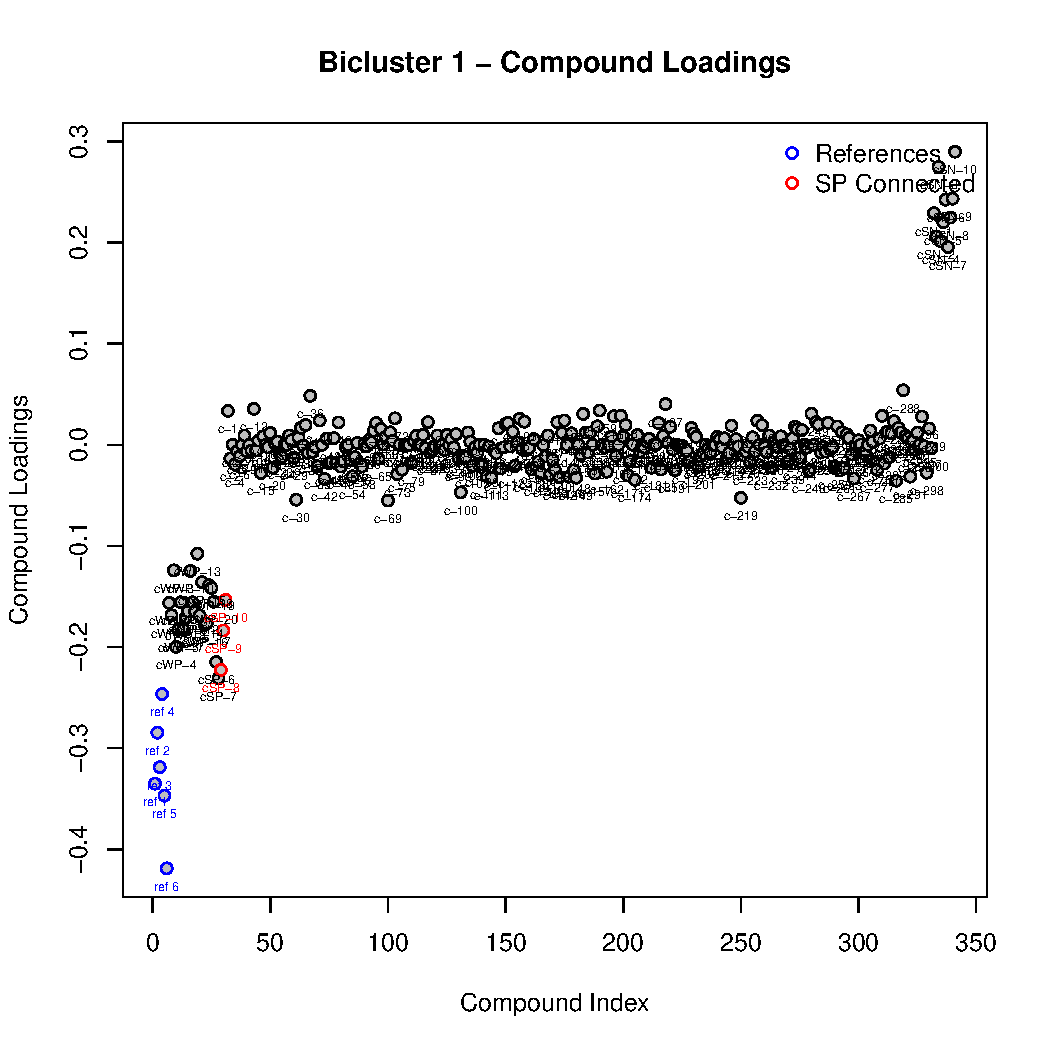
\includegraphics[width=9cm,height=10cm]{figure/FABIA-2} 
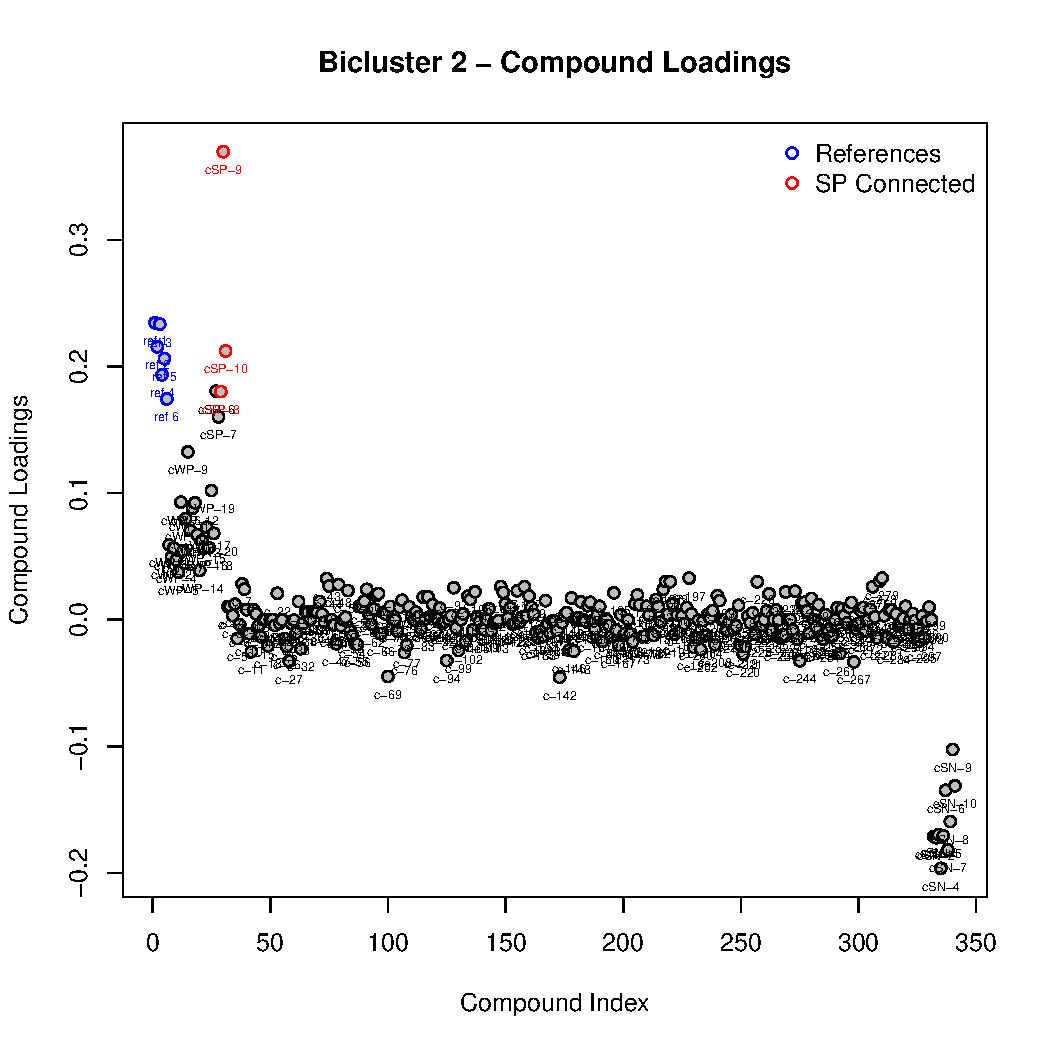
\includegraphics[width=9cm,height=10cm]{figure/FABIA-3} \hfill{}

\caption[CSanalysis Graphs for CSfabia]{CSanalysis Graphs for CSfabia\label{fig:FABIA}}
\end{figure}


\end{knitrout}
\noindent The results in Figure \ref{fig:FABIA} are very comparable with the
Zhang and MFA graphs.
% 23,24,25 -> 29,30,31
%highlight the connected ones in MFA, look if the same ones (hurrdurr)

\section{Example CS permutation}
The \texttt{CSFA} package also contains a function called \texttt{CSpermute}.
With this function it is possible to compute p-values through permutation for
the MFA and Zhang \& Gant results. \\
These results will be added to the \verb|CS| slot of both the MFA and ZG
results. More information is also entered in the \verb|permutation.object| slot. 
\\ \\
First, let us apply the permutation on the MFA and ZG result without plotting
any plots just yet by putting \texttt{which} to \texttt{c()}. The number of
permutation was chosen to only be 100 in this case. Further, the p-values are
also adjusted for multiplicity by setting a value for \texttt{method.adjust}
different than \texttt{"none"}.\\
(Note: it is possible for MFA results to compute the p-values in a different factor than the one chosen in the CS analysis. This is accomplished through the \texttt{mfa.factor} parameter.)


\begin{knitrout}
\definecolor{shadecolor}{rgb}{0.969, 0.969, 0.969}\color{fgcolor}\begin{kframe}
\begin{alltt}
        \hlstd{out_MFA} \hlkwb{<-} \hlkwd{CSpermute}\hlstd{(refMat,querMat,}\hlkwc{CSresult}\hlstd{=out_MFA,}\hlkwc{B}\hlstd{=}\hlnum{100}\hlstd{,}\hlkwc{method.adjust}\hlstd{=}\hlstr{"BH"}\hlstd{,}
                        \hlkwc{which}\hlstd{=}\hlkwd{c}\hlstd{(),}\hlkwc{verbose}\hlstd{=}\hlnum{FALSE}\hlstd{)}
        \hlstd{out_ZG} \hlkwb{<-} \hlkwd{CSpermute}\hlstd{(refMat,querMat,}\hlkwc{CSresult}\hlstd{=out_ZG,}\hlkwc{B}\hlstd{=}\hlnum{100}\hlstd{,}\hlkwc{method.adjust}\hlstd{=}\hlstr{"BH"}\hlstd{,}
                        \hlkwc{which}\hlstd{=}\hlkwd{c}\hlstd{(),}\hlkwc{verbose}\hlstd{=}\hlnum{FALSE}\hlstd{)}
\end{alltt}
\end{kframe}
\end{knitrout}


\begin{knitrout}
\definecolor{shadecolor}{rgb}{0.969, 0.969, 0.969}\color{fgcolor}\begin{kframe}
\begin{alltt}
\hlkwd{head}\hlstd{(out_MFA}\hlopt{@}\hlkwc{CS}\hlopt{$}\hlstd{CS.query)}
\end{alltt}
\begin{verbatim}
##         Factor1 pvalues pvalues.adjusted
## cWP-1 0.5858096       0                0
## cWP-2 0.5771857       0                0
## cWP-3 0.5739775       0                0
## cWP-4 0.5867910       0                0
## cWP-5 0.5770335       0                0
## cWP-6 0.5852554       0                0
\end{verbatim}
\begin{alltt}
\hlkwd{head}\hlstd{(out_ZG}\hlopt{@}\hlkwc{CS}\hlopt{$}\hlstd{CS.query)}
\end{alltt}
\begin{verbatim}
##       ZhangScore pvalues pvalues.adjusted
## cWP-1  0.5590061       0                0
## cWP-2  0.5473340       0                0
## cWP-3  0.5621351       0                0
## cWP-4  0.5649765       0                0
## cWP-5  0.5578107       0                0
## cWP-6  0.5468158       0                0
\end{verbatim}
\end{kframe}
\end{knitrout}

\noindent Next, we can actually re-use the updated \texttt{out\_MFA} and
\texttt{out\_ZG} in \texttt{CSpermute}.
As long as the number of permutations (\texttt{B}) is not changed, the permutation will not need to computed all over again. 
This means you can plot the available graphs (\text{which}: 1, volcano plot ; 2, connectivity score compound distribution histogram under null hypothesis with p-value) as many times as needed.
The parameter \texttt{cmpd.hist} decides which compounds should be used for the second type of plot. 
If this parameter is not given (\texttt{NULL}), you can interactively choose them on the volcano plot by left-clicking on them (and right-click to stop).
In the code below, we plot both type of graphs for the MFA result with a pre-determined \texttt{cmpd.hist}.

\begin{knitrout}
\definecolor{shadecolor}{rgb}{0.969, 0.969, 0.969}\color{fgcolor}\begin{kframe}
\begin{alltt}
\hlstd{out_MFA} \hlkwb{<-} \hlkwd{CSpermute}\hlstd{(refMat,querMat,out_MFA,}\hlkwc{B}\hlstd{=}\hlnum{100}\hlstd{,}\hlkwc{method.adjust}\hlstd{=}\hlstr{"BH"}\hlstd{,}
                \hlkwc{which}\hlstd{=}\hlkwd{c}\hlstd{(}\hlnum{1}\hlstd{,}\hlnum{2}\hlstd{),}\hlkwc{cmpd.hist}\hlstd{=}\hlkwd{c}\hlstd{(}\hlnum{29}\hlstd{,}\hlnum{105}\hlstd{),}\hlkwc{plot.type}\hlstd{=}\hlstr{"sweave"}\hlstd{)}
\end{alltt}
\end{kframe}\begin{figure}[H]


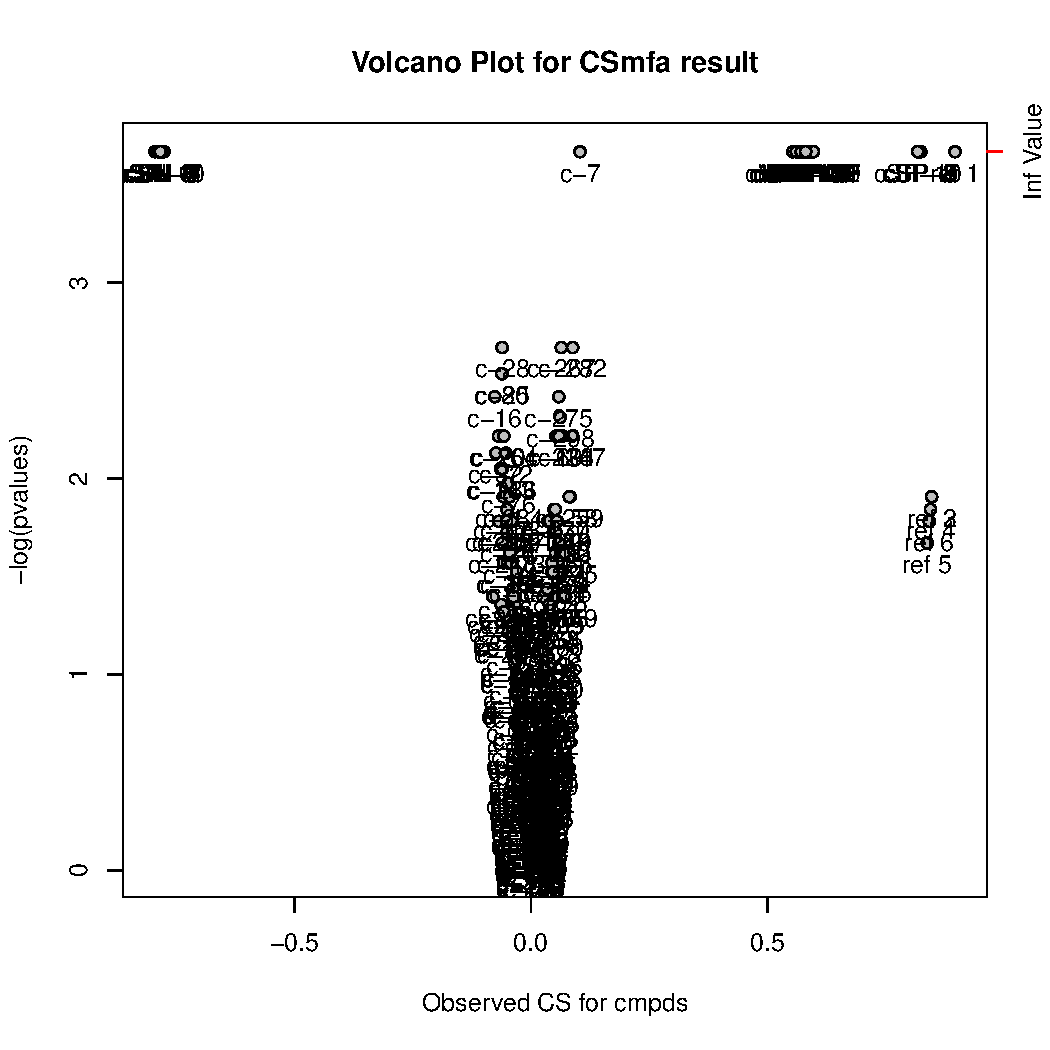
\includegraphics[width=9cm,height=10cm]{figure/CSpermute_plots-1} 
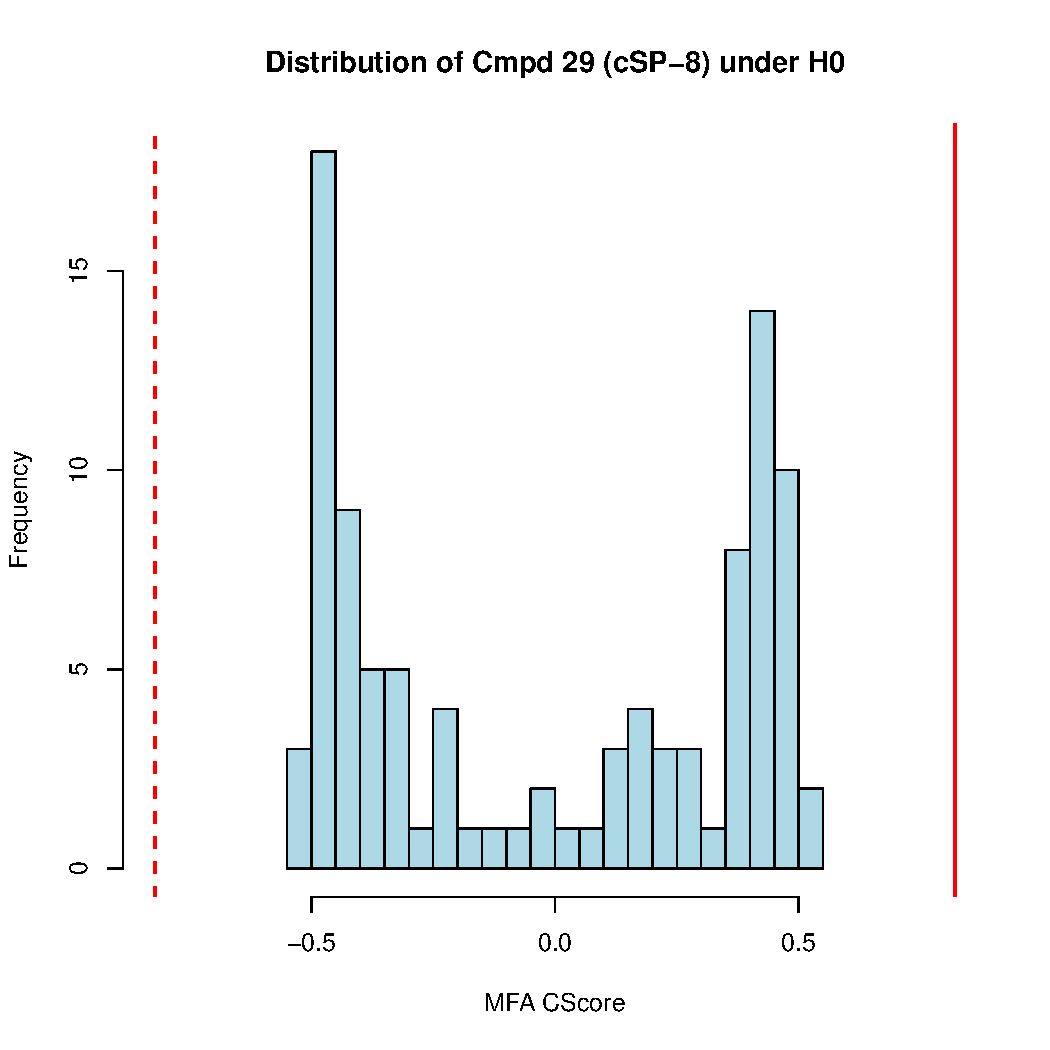
\includegraphics[width=9cm,height=10cm]{figure/CSpermute_plots-2} 
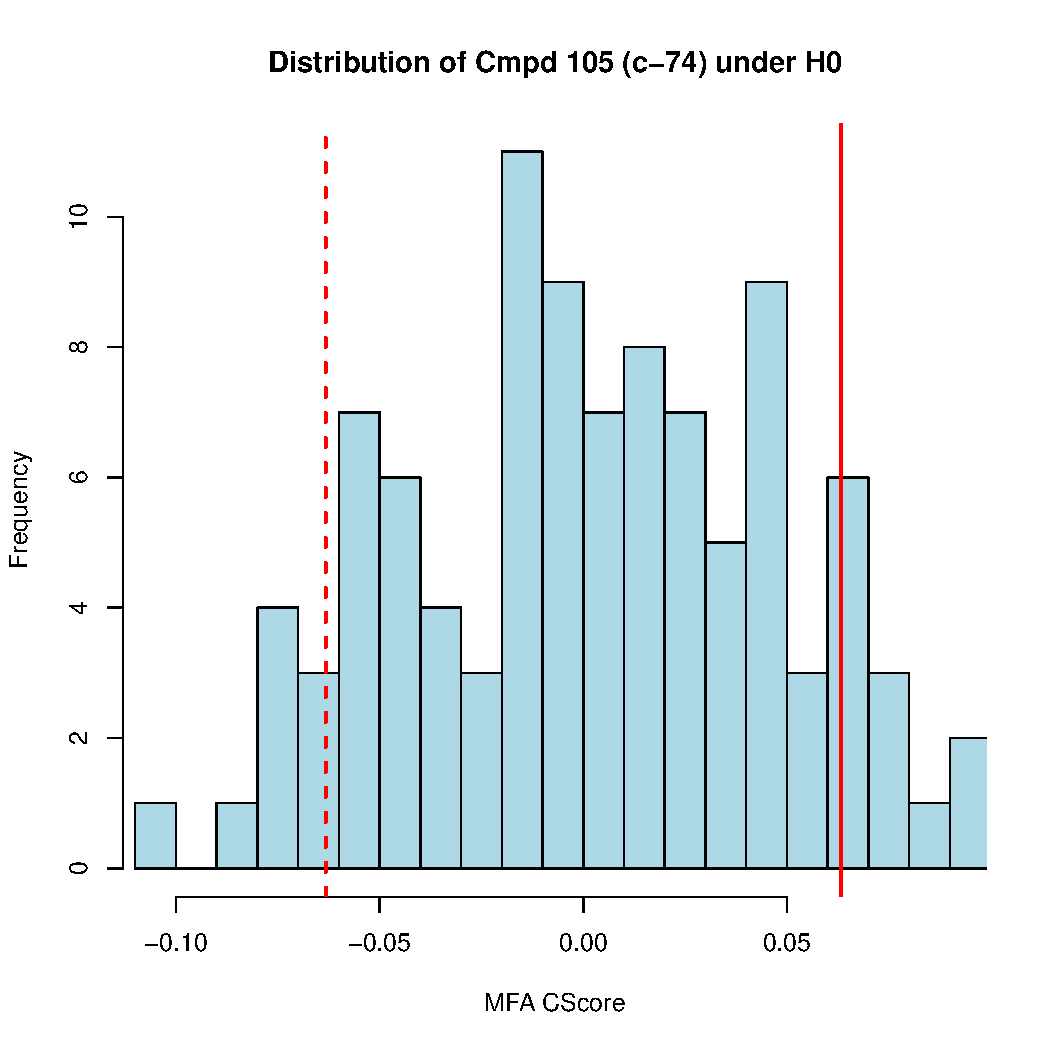
\includegraphics[width=9cm,height=10cm]{figure/CSpermute_plots-3} \hfill{}

\caption[CSpermute graphs for out_MFA]{CSpermute graphs for out_MFA\label{fig:CSpermute_plots}}
\end{figure}


\end{knitrout}

\section{Example Compare CS Results}
Finally, CSFA also provides a way to quickly compare the 2 results on the same
data.\\
In the R-code below, we first compare the Zhang and Gant results with the MFA
result. With \texttt{component2.plot=1} we choose the first component for the
second result which is the first factor for the MFA result in this example.
Since the Zhang and Gant analysis only provides connectivity scores, only 1
comparison graph will be created.\\
The second example in the code compares the MFA with the FABIA results. For both
results we choose the first component which corresponds with the first factor
and first bicluster. Further, we also set some positive and negative gene
thresholds for both of the results. In this example we keep them the same for
both the MFA and FABIA results namely 2 for the upper threshold and -2 for the
lower one. This time since both results also contain gene scores, 2 graphs will
be created. Further because we set thresholds for the genes, the gene score
comparison plot will be coloring according to these thresholds.

\begin{knitrout}
\definecolor{shadecolor}{rgb}{0.969, 0.969, 0.969}\color{fgcolor}\begin{kframe}
\begin{alltt}
        \hlstd{corr_ZG_MFA} \hlkwb{<-} \hlkwd{CScompare}\hlstd{(out_ZG,out_MFA,}\hlkwc{component2.plot}\hlstd{=}\hlnum{1}\hlstd{,}\hlkwc{plot.type}\hlstd{=}\hlstr{"sweave"}\hlstd{)}

        \hlstd{corr_MFA_FABIA} \hlkwb{<-} \hlkwd{CScompare}\hlstd{(out_MFA,out_FABIA,}\hlkwc{component1.plot}\hlstd{=}\hlnum{1}\hlstd{,}\hlkwc{component2.plot}\hlstd{=}\hlnum{1}\hlstd{,}
                        \hlkwc{gene.thresP}\hlstd{=}\hlkwd{c}\hlstd{(}\hlnum{2}\hlstd{,}\hlnum{2}\hlstd{),}\hlkwc{gene.thresN}\hlstd{=}\hlkwd{c}\hlstd{(}\hlopt{-}\hlnum{2}\hlstd{,}\hlopt{-}\hlnum{2}\hlstd{),}\hlkwc{plot.type}\hlstd{=}\hlstr{"sweave"}\hlstd{)}

        \hlstd{corr_ZG_MFA}\hlopt{$}\hlstd{correlation}
\end{alltt}
\begin{verbatim}
## CS Correlation 
##      0.9931169
\end{verbatim}
\begin{alltt}
        \hlstd{corr_MFA_FABIA}\hlopt{$}\hlstd{correlation}
\end{alltt}
\begin{verbatim}
## CS Correlation GS Correlation 
##     -0.9573119     -0.7752930
\end{verbatim}
\end{kframe}\begin{figure}[H]


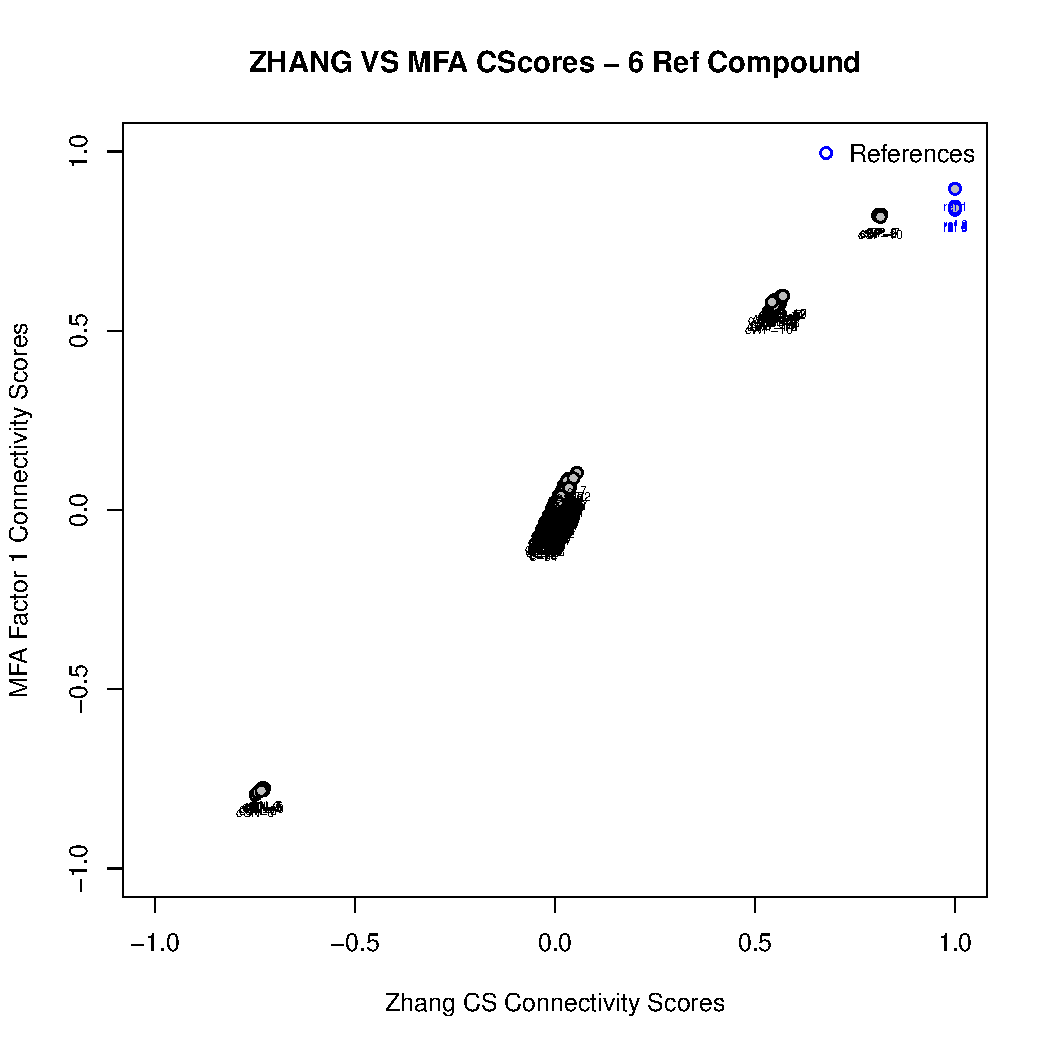
\includegraphics[width=9cm,height=10cm]{figure/CScompare-1} 
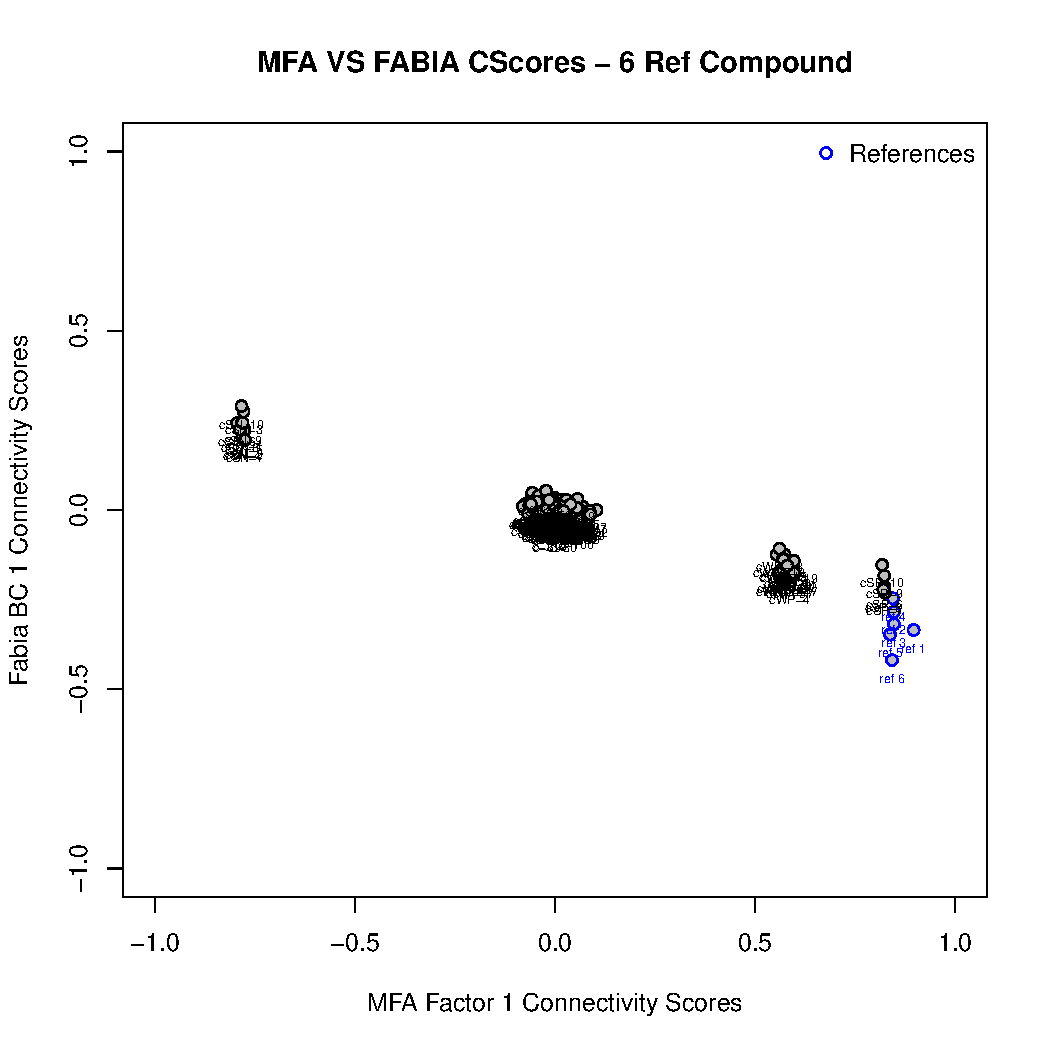
\includegraphics[width=9cm,height=10cm]{figure/CScompare-2} 
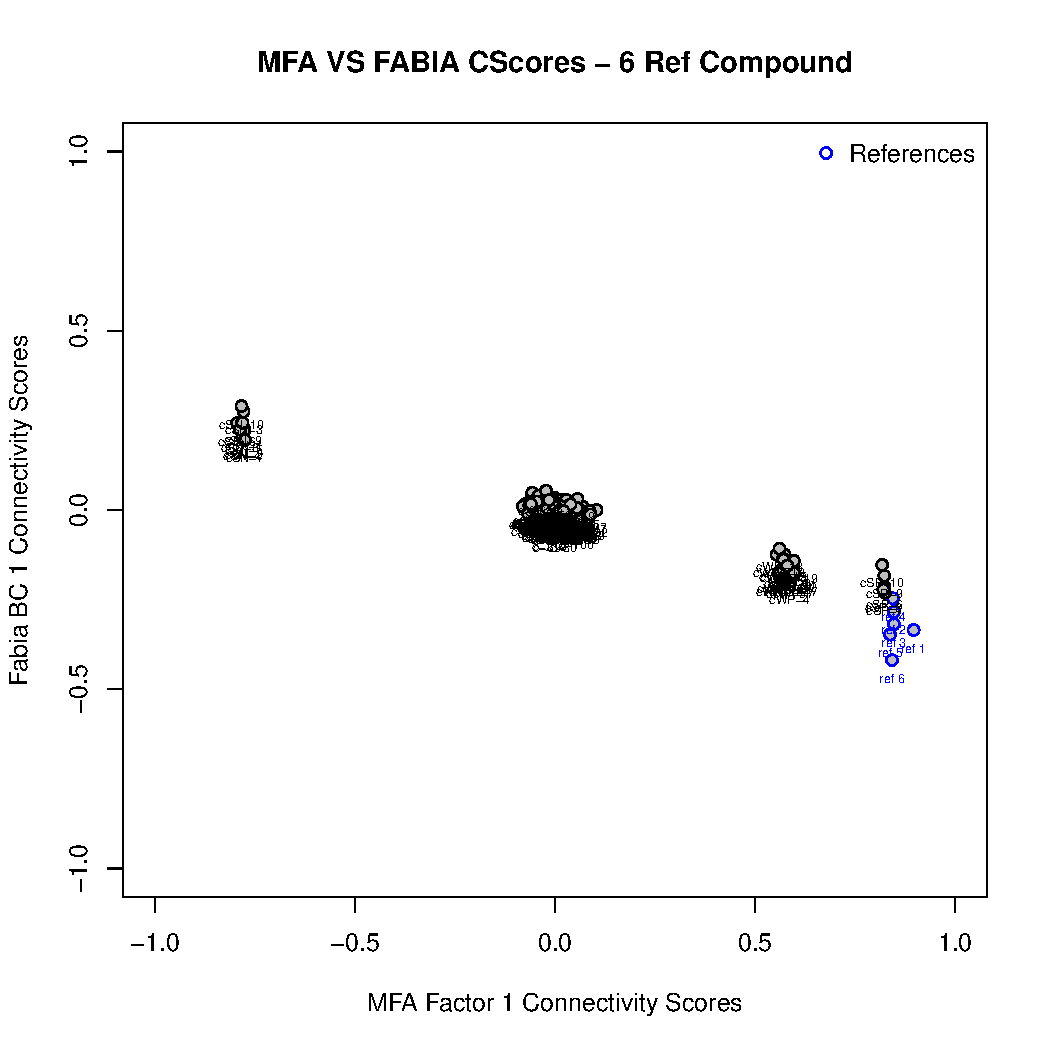
\includegraphics[width=9cm,height=10cm]{figure/CScompare-3} \hfill{}

\caption[Compare CSresults]{Compare CSresults\label{fig:CScompare}}
\end{figure}


\end{knitrout}
\noindent Note that apart from the scatter plots in Figure \ref{fig:CScompare},
the function also returns the pearson correlation between the scores.
\\ \\
Further because both the MFA and ZG contain p-values and adjusted p-values, the
returned object also contains a small comparison between the number of
significant p-values. The significancy threshold can be changed with the
\texttt{threshold.pvalues} parameter and is defaulted to 0.05.
\begin{knitrout}
\definecolor{shadecolor}{rgb}{0.969, 0.969, 0.969}\color{fgcolor}\begin{kframe}
\begin{alltt}
        \hlstd{corr_ZG_MFA}\hlopt{$}\hlstd{compare.pvalues}
\end{alltt}
\begin{verbatim}
##                 Result1.Sign Result1.NotSign
## Result2.Sign              37               0
## Result2.NotSign           47             257
\end{verbatim}
\begin{alltt}
        \hlstd{corr_ZG_MFA}\hlopt{$}\hlstd{compare.pvalues.adjusted}
\end{alltt}
\begin{verbatim}
##                 Result1.Sign Result1.NotSign
## Result2.Sign              37               0
## Result2.NotSign           11             293
\end{verbatim}
\end{kframe}
\end{knitrout}

\newpage
%\nocite{*}
\bibliographystyle{asa}
\bibliography{connectivityRef}


\end{document}
